\documentclass[12pt,tikz]{standalone}
\pdfinfoomitdate 1
\pdfsuppressptexinfo 1
\pdftrailerid{}
\usepackage[utf8]{inputenc}
\usepackage{amsmath}
\usepackage{pgfplots}
\usepackage{tikz}
\pagestyle{empty}

\begin{document}
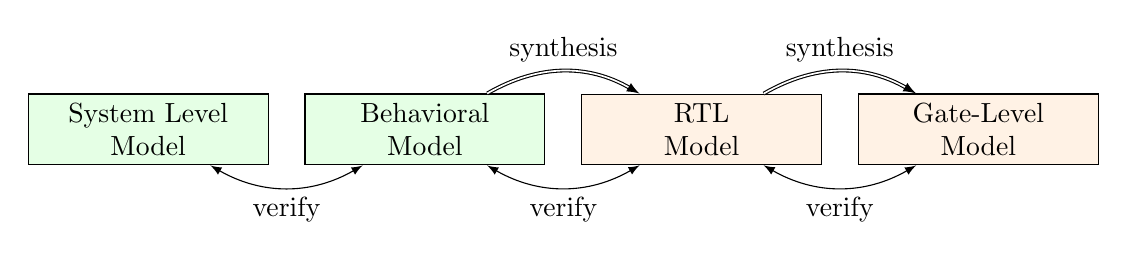
\begin{tikzpicture}
	\tikzstyle{manual} = [draw, fill=green!10, rectangle, minimum height=2em, minimum width=8em, node distance=10em]
	\tikzstyle{auto} = [draw, fill=orange!10, rectangle, minimum height=2em, minimum width=8em, node distance=10em]

	\node[manual] (sys) {\begin{minipage}{8em}
		\center
		System Level \\
		Model
	\end{minipage}};
	\node[manual] (beh) [right of=sys] {\begin{minipage}{8em}
		\center
		Behavioral \\
		Model
	\end{minipage}};
	\node[auto] (rtl) [right of=beh] {\begin{minipage}{8em}
		\center
		RTL \\
		Model
	\end{minipage}};
	\node[auto] (gates) [right of=rtl] {\begin{minipage}{8em}
		\center
		Gate-Level \\
		Model
	\end{minipage}};

	\draw[-latex] (beh) edge[double, bend left] node[above] {synthesis} (rtl);
	\draw[-latex] (rtl) edge[double, bend left] node[above] {synthesis} (gates);

	\draw[latex-latex] (sys) edge[bend right] node[below] {verify} (beh);
	\draw[latex-latex] (beh) edge[bend right] node[below] {verify} (rtl);
	\draw[latex-latex] (rtl) edge[bend right] node[below] {verify} (gates);
\end{tikzpicture}
\end{document}
